\setcounter{chapter}{3}
\chapter{Conclusion and Future Work}
In this chapter, we describe the phases of our plan for exploring the research challenges and investigating the research issues identified in Chapter 4. This chapter also includes research methodology and future publication plan.

\section {Conclusion}

In this report, we proposed a cooperative game theory-based model
for the aggregation of web services within communities. The goal
of our services is to maximize efficiency by collaborating and
forming stable coalitions. Our method considers stability and
fairness for all web services within a community and offers an
applicable mechanism for membership requests and selection of web
services. The ultimate goal is to increase revenue by improving
user satisfaction, which comes from the ability to perform more
tasks with high quality. Simulation results show that our,
polynomial in complexity, approximation algorithms provide web
services and community owners with applicable and near-optimal
decision making mechanisms.

%As future work, we would like to perform more analytical and
%theoretical analysis on the convexity condition and also minimal $\epsilon$ values in \emph{$\epsilon$-core} solution concepts based on the
%characteristic function in web service applications. From web service perspective, the
%work can be extended to consider web service compositions where a
%group of web services having different set of skills cooperate to
%perform composite tasks. Also bargaining theory from cooperating
%game theory concepts can be used to help web services resolve the
%instability and unfairness issues by side payments.

\section {Future Plan and Timeline}

\indent The future goals in this PhD research work mainly consists of:

\begin{itemize}
\item Analysing other cooperative solution concepts such as Kernel and Nucleolus where payoff division is guaranteed to exist but may have optimal results.
\item Applying Weighted Voting Games (WCG) type of valuation function in our scenarios, Developing a multiple weighted algorithm to find best coalition structures satisfying different weights on each community.
\item Implementing Q-learning and reinforcement learning technique and also a tic-tac-toe based repeated game technique for individual Web Service decision making process, in long term and repeated game scenarios.
\item Developing an approximation algorithm for shapely value payoff distribution vector in community of service setting.    
\item Developing a community membership algorithm technique for our agents in "incomplete information" settings.
\item Developing an open source, Java based Tool, with UI for solving Core and Shapely solution concepts based on different input valuation functions.
\end{itemize}


    \begin{figure}
                \begin{center}
%                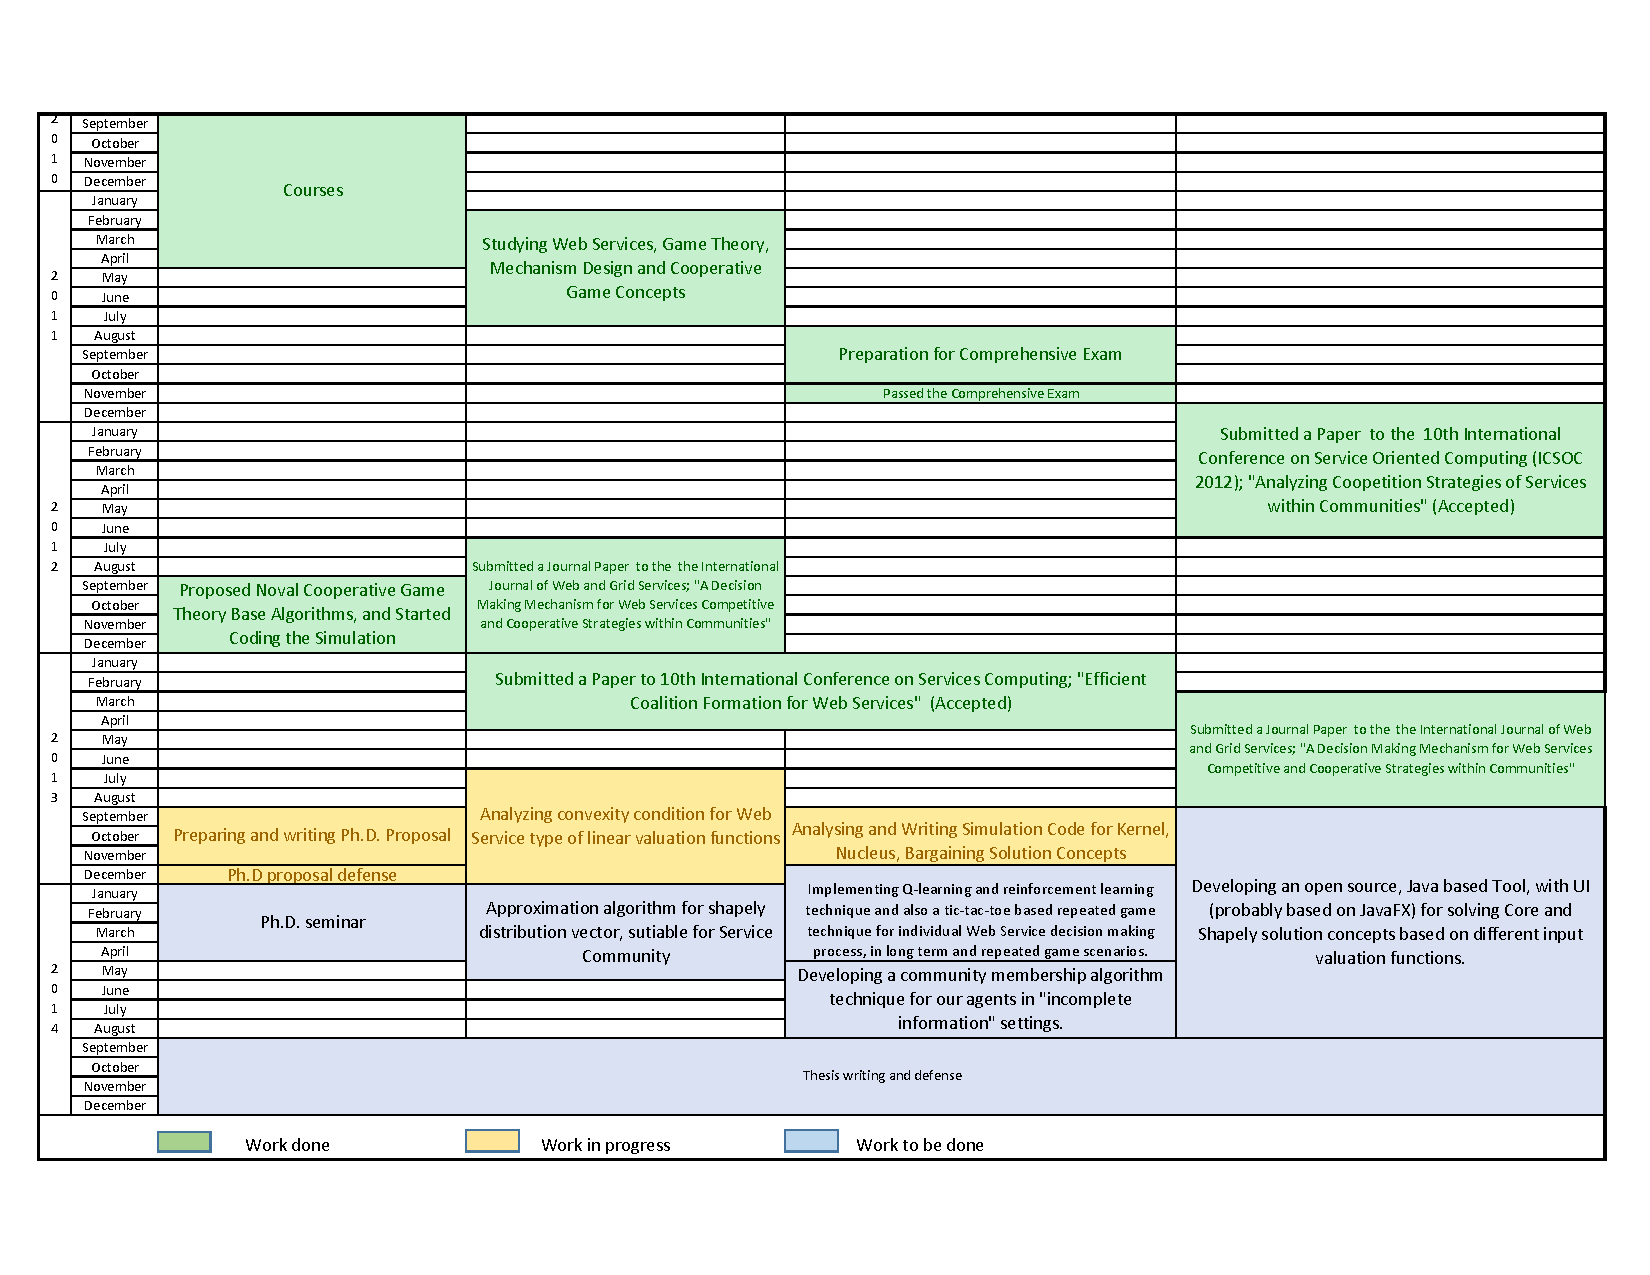
\includegraphics[width=16cm, height=22cm]{timeline/timetable.pdf}\label{Timetable}
                \includegraphics[width=16cm]{Figures/fw.eps}\label{Timetable}
                \caption{Research milestones and time line}
                \end{center}
    \end{figure}   